\begin{enumerate}[label=\thesubsection.\arabic*.,ref=\thesubsection.\theenumi]
\numberwithin{equation}{enumi}

\item Tabulate the transfer functions of a PID controller and its variants.
\\
\solution See Table \ref{table:ee18btech11021}.

\begin{table}[!ht]
\centering
%%%%%%%%%%%%%%%%%%%%%%%%%%%%%%%%%%%%%%%%%%%%%%%%%%%%%%%%%%%%%%%%%%%%%%
%%                                                                  %%
%%  This is the header of a LaTeX2e file exported from Gnumeric.    %%
%%                                                                  %%
%%  This file can be compiled as it stands or included in another   %%
%%  LaTeX document. The table is based on the longtable package so  %%
%%  the longtable options (headers, footers...) can be set in the   %%
%%  preamble section below (see PRAMBLE).                           %%
%%                                                                  %%
%%  To include the file in another, the following two lines must be %%
%%  in the including file:                                          %%
%%        \def\inputGnumericTable{}                                 %%
%%  at the beginning of the file and:                               %%
%%        \input{name-of-this-file.tex}                             %%
%%  where the table is to be placed. Note also that the including   %%
%%  file must use the following packages for the table to be        %%
%%  rendered correctly:                                             %%
%%    \usepackage[latin1]{inputenc}                                 %%
%%    \usepackage{color}                                            %%
%%    \usepackage{array}                                            %%
%%    \usepackage{longtable}                                        %%
%%    \usepackage{calc}                                             %%
%%    \usepackage{multirow}                                         %%
%%    \usepackage{hhline}                                           %%
%%    \usepackage{ifthen}                                           %%
%%  optionally (for landscape tables embedded in another document): %%
%%    \usepackage{lscape}                                           %%
%%                                                                  %%
%%%%%%%%%%%%%%%%%%%%%%%%%%%%%%%%%%%%%%%%%%%%%%%%%%%%%%%%%%%%%%%%%%%%%%



%%  This section checks if we are begin input into another file or  %%
%%  the file will be compiled alone. First use a macro taken from   %%
%%  the TeXbook ex 7.7 (suggestion of Han-Wen Nienhuys).            %%
\def\ifundefined#1{\expandafter\ifx\csname#1\endcsname\relax}


%%  Check for the \def token for inputed files. If it is not        %%
%%  defined, the file will be processed as a standalone and the     %%
%%  preamble will be used.                                          %%
\ifundefined{inputGnumericTable}

%%  We must be able to close or not the document at the end.        %%
	\def\gnumericTableEnd{\end{document}}


%%%%%%%%%%%%%%%%%%%%%%%%%%%%%%%%%%%%%%%%%%%%%%%%%%%%%%%%%%%%%%%%%%%%%%
%%                                                                  %%
%%  This is the PREAMBLE. Change these values to get the right      %%
%%  paper size and other niceties.                                  %%
%%                                                                  %%
%%%%%%%%%%%%%%%%%%%%%%%%%%%%%%%%%%%%%%%%%%%%%%%%%%%%%%%%%%%%%%%%%%%%%%

	\documentclass[12pt%
			  %,landscape%
                    ]{report}
       \usepackage[latin1]{inputenc}
       \usepackage{fullpage}
       \usepackage{color}
       \usepackage{array}
       \usepackage{longtable}
       \usepackage{calc}
       \usepackage{multirow}
       \usepackage{hhline}
       \usepackage{ifthen}

	\begin{document}


%%  End of the preamble for the standalone. The next section is for %%
%%  documents which are included into other LaTeX2e files.          %%
\else

%%  We are not a stand alone document. For a regular table, we will %%
%%  have no preamble and only define the closing to mean nothing.   %%
    \def\gnumericTableEnd{}

%%  If we want landscape mode in an embedded document, comment out  %%
%%  the line above and uncomment the two below. The table will      %%
%%  begin on a new page and run in landscape mode.                  %%
%       \def\gnumericTableEnd{\end{landscape}}
%       \begin{landscape}


%%  End of the else clause for this file being \input.              %%
\fi

%%%%%%%%%%%%%%%%%%%%%%%%%%%%%%%%%%%%%%%%%%%%%%%%%%%%%%%%%%%%%%%%%%%%%%
%%                                                                  %%
%%  The rest is the gnumeric table, except for the closing          %%
%%  statement. Changes below will alter the table's appearance.     %%
%%                                                                  %%
%%%%%%%%%%%%%%%%%%%%%%%%%%%%%%%%%%%%%%%%%%%%%%%%%%%%%%%%%%%%%%%%%%%%%%

\providecommand{\gnumericmathit}[1]{#1} 
%%  Uncomment the next line if you would like your numbers to be in %%
%%  italics if they are italizised in the gnumeric table.           %%
%\renewcommand{\gnumericmathit}[1]{\mathit{#1}}
\providecommand{\gnumericPB}[1]%
{\let\gnumericTemp=\\#1\let\\=\gnumericTemp\hspace{0pt}}
 \ifundefined{gnumericTableWidthDefined}
        \newlength{\gnumericTableWidth}
        \newlength{\gnumericTableWidthComplete}
        \newlength{\gnumericMultiRowLength}
        \global\def\gnumericTableWidthDefined{}
 \fi
%% The following setting protects this code from babel shorthands.  %%
 \ifthenelse{\isundefined{\languageshorthands}}{}{\languageshorthands{english}}
%%  The default table format retains the relative column widths of  %%
%%  gnumeric. They can easily be changed to c, r or l. In that case %%
%%  you may want to comment out the next line and uncomment the one %%
%%  thereafter                                                      %%
\providecommand\gnumbox{\makebox[0pt]}
%%\providecommand\gnumbox[1][]{\makebox}

%% to adjust positions in multirow situations                       %%
\setlength{\bigstrutjot}{\jot}
\setlength{\extrarowheight}{\doublerulesep}

%%  The \setlongtables command keeps column widths the same across  %%
%%  pages. Simply comment out next line for varying column widths.  %%
\setlongtables

\setlength\gnumericTableWidth{%
	53pt+%
	93pt+%
0pt}
\def\gumericNumCols{2}
\setlength\gnumericTableWidthComplete{\gnumericTableWidth+%
         \tabcolsep*\gumericNumCols*2+\arrayrulewidth*\gumericNumCols}
\ifthenelse{\lengthtest{\gnumericTableWidthComplete > \linewidth}}%
         {\def\gnumericScale{\ratio{\linewidth-%
                        \tabcolsep*\gumericNumCols*2-%
                        \arrayrulewidth*\gumericNumCols}%
{\gnumericTableWidth}}}%
{\def\gnumericScale{1}}

%%%%%%%%%%%%%%%%%%%%%%%%%%%%%%%%%%%%%%%%%%%%%%%%%%%%%%%%%%%%%%%%%%%%%%
%%                                                                  %%
%% The following are the widths of the various columns. We are      %%
%% defining them here because then they are easier to change.       %%
%% Depending on the cell formats we may use them more than once.    %%
%%                                                                  %%
%%%%%%%%%%%%%%%%%%%%%%%%%%%%%%%%%%%%%%%%%%%%%%%%%%%%%%%%%%%%%%%%%%%%%%

\ifthenelse{\isundefined{\gnumericColA}}{\newlength{\gnumericColA}}{}\settowidth{\gnumericColA}{\begin{tabular}{@{}p{53pt*\gnumericScale}@{}}x\end{tabular}}
\ifthenelse{\isundefined{\gnumericColB}}{\newlength{\gnumericColB}}{}\settowidth{\gnumericColB}{\begin{tabular}{@{}p{93pt*\gnumericScale}@{}}x\end{tabular}}

\begin{tabular}[c]{%
	b{\gnumericColA}%
	b{\gnumericColB}%
	}

%%%%%%%%%%%%%%%%%%%%%%%%%%%%%%%%%%%%%%%%%%%%%%%%%%%%%%%%%%%%%%%%%%%%%%
%%  The longtable options. (Caption, headers... see Goosens, p.124) %%
%	\caption{The Table Caption.}             \\	%
% \hline	% Across the top of the table.
%%  The rest of these options are table rows which are placed on    %%
%%  the first, last or every page. Use \multicolumn if you want.    %%

%%  Header for the first page.                                      %%
%	\multicolumn{2}{c}{The First Header} \\ \hline 
%	\multicolumn{1}{c}{colTag}	%Column 1
%	&\multicolumn{1}{c}{colTag}	\\ \hline %Last column
%	\endfirsthead

%%  The running header definition.                                  %%
%	\hline
%	\multicolumn{2}{l}{\ldots\small\slshape continued} \\ \hline
%	\multicolumn{1}{c}{colTag}	%Column 1
%	&\multicolumn{1}{c}{colTag}	\\ \hline %Last column
%	\endhead

%%  The running footer definition.                                  %%
%	\hline
%	\multicolumn{2}{r}{\small\slshape continued\ldots} \\
%	\endfoot

%%  The ending footer definition.                                   %%
%	\multicolumn{2}{c}{That's all folks} \\ \hline 
%	\endlastfoot
%%%%%%%%%%%%%%%%%%%%%%%%%%%%%%%%%%%%%%%%%%%%%%%%%%%%%%%%%%%%%%%%%%%%%%

\hhline{|-|-}
	 \multicolumn{1}{|p{\gnumericColA}|}%
	{\gnumericPB{\centering}\gnumbox{\textbf{Controller}}}
	&\multicolumn{1}{p{\gnumericColB}|}%
	{\gnumericPB{\centering}\gnumbox{\textbf{Gain}}}
\\
\hhline{|--|}
	 \multicolumn{1}{|p{\gnumericColA}|}%
	{\gnumericPB{\centering}\gnumbox{PID}}
	&\multicolumn{1}{p{\gnumericColB}|}%
	{$    K_{p}\brak{1 + T_{d}s + \frac{1}{T_{i}s}}$}
\\
\hhline{|--|}
	 \multicolumn{1}{|p{\gnumericColA}|}%
	{\gnumericPB{\centering}\gnumbox{PD}}
	&\multicolumn{1}{p{\gnumericColB}|}%
	{$    K_{p}(1 + T_{d}s)$}
\\
\hhline{|--|}
	 \multicolumn{1}{|p{\gnumericColA}|}%
	{\gnumericPB{\centering}\gnumbox{PI}}
	&\multicolumn{1}{p{\gnumericColB}|}%
	{$    K_{p}\brak{1 +  \frac{1}{T_{i}s}}$}
\\
\hhline{|-|-|}
\end{tabular}

\ifthenelse{\isundefined{\languageshorthands}}{}{\languageshorthands{\languagename}}
\gnumericTableEnd

\caption{}
\label{table:ee18btech11021}
\end{table}


\item
For a unity Feedback system 
\begin{align}
    G(s) = \frac{K}{s(s+2)(s+4)(s+6)}
\end{align}
%
Design a PD Controller with $K_{v} = 2$ and Phase Margin 30\degree

\solution The gain after cascading the PD Controller with  G(s) is 
%
\begin{align}
    G_{c}(s) = \frac{K_{p}(1 + T_{d}s)K}{s(s+2)(s+4)(s+6)}
\label{eq:ee18btech11021}
\end{align}
%
Choosing  $K_{p} = 1$ in \label{eq:ee18btech11021},
%
\begin{align}
    K_{v} &= \lim_{s \to 0} sG_{c}(s) = 2
\\
    \implies K &= 96
\end{align}

For Phase Margin 30\degree, at Gain Crossover Frequency $\omega$,
%
\begin{multline}
    \tan^{-1}\brak{T_{d}\omega} - \tan^{-1}\brak{\frac{\omega}{2}} - \tan^{-1}\brak{\frac{\omega}{4}}
\\
-    \tan^{-1}\brak{\frac{\omega}{6}} = -60 \degree
\end{multline}

\begin{align}
    \abs{G_{1}\brak{\j\omega}} = \frac{96\sqrt{T_{d}^2\omega^2 + 1}}{\omega\sqrt{(\omega^2+4)(\omega^2 + 16)(\omega^2 + 36)}} = 1
\end{align}

By Hit and Trial, one of the best combinations is
\begin{align}
    \omega = 4
\end{align}
\begin{align}
    T_{d} = 1.884
\end{align}
We get a Phase Margin of 30.31\degree

\item
Verify using a Python Plot

\solution The following code plots Fig. \ref{fig:ee18btech11021_pd}

\begin{lstlisting}
codes/ee18btech11021/EE18BTECH11021_3.py
\end{lstlisting}

\begin{figure}[!ht]
\centering
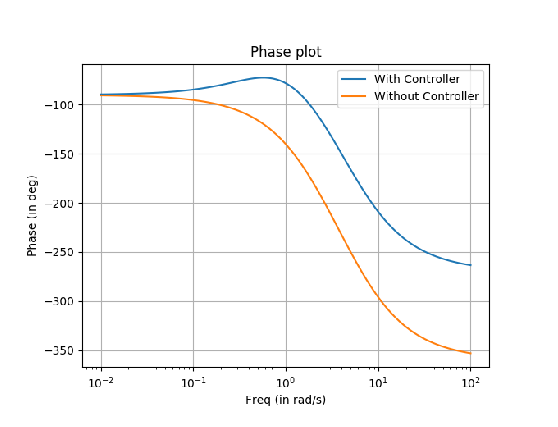
\includegraphics[width=\columnwidth]{./figs/ee18btech11021/EE18BTECH11021_PD.eps}
\caption{}
\label{fig:ee18btech11021_pd}
\end{figure}

\item
Design a PI Controller with $K_{v} = \infty$ and Phase Margin 30\degree

\solution From Table \ref{table:ee18btech11021}, the open loop gain in this case is

\begin{align}
    G_{1}(s) = \frac{K_{p}\brak{1 +  \frac{1}{T_{i}s}}K}{s(s+2)(s+4)(s+6)}
\end{align}

Choose $K_{p}K = 96$. Then
\begin{align}
    G_{1}(s) = \frac{96(T_{i}s + 1)}{T_{i}s^2(s+2)(s+4)(s+6)}
\end{align}

For Phase Margin 30\degree, at Gain Crossover Frequency $\omega$

\begin{multline}
    \tan^{-1}(T_{i}\omega) - \tan^{-1}\brak{\frac{\omega}{2}} - \tan^{-1}\brak{\frac{\omega}{4}}
\\
-    \tan^{-1}\brak{\frac{\omega}{6}} = 30
\end{multline}
and
\begin{align}
    \abs{G_{1}\brak{\j\omega}} = \frac{96\sqrt{T_{i}^2\omega^2 + 1}}{T_{i}^2\omega^2\sqrt{(\omega^2+4)(\omega^2 + 16)(\omega^2 + 36)}} = 1
\end{align}

By Hit and Trial, one of the best combinations is
\begin{align}
    \omega &= 0.75
\\
    T_{i} &= 2.713
\end{align}
We get a Phase Margin of 25.53\degree

\item
Verify using a Python Plot

\solution The following code plots Fig. \ref{fig:ee18btech11021_pi}.

\begin{lstlisting}
codes/ee18btech11021/EE18BTECH11021_4.py
\end{lstlisting}

\begin{figure}[!ht]
\centering
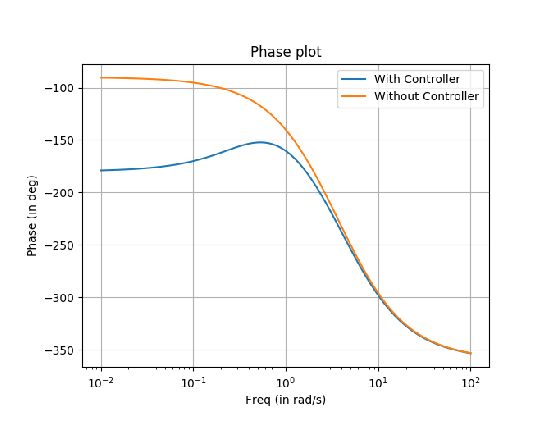
\includegraphics[width=\columnwidth]{./figs/ee18btech11021/EE18BTECH11021_PI.eps}
\caption{}
\label{fig:ee18btech11021_pi}
\end{figure}

\item
Design a PID Controller with $K_{v} = \infty$ and Phase Margin 30\degree

\solution

\begin{align}
    G_{1}(s) = \frac{K_{p}\brak{1 + T_{d}s + \frac{1}{T_{i}s}}K}{s(s+2)(s+4)(s+6)}
\end{align}

Choose $K_{p}K = 96$.  The open loop gain is
\begin{align}
    G_{1}(s) = \frac{96(T_{i}T_{d}s^2 + T_{i}s +  1)}{T_{i}s^2(s+2)(s+4)(s+6)}
\end{align}

For Phase Margin 30\degree, at Gain Crossover Frequency $\omega$,

\begin{multline}
    \tan^{-1}\brak{\frac{T_{i}\omega}{1-T{i}T_{d}w^2}} - \tan^{-1}\brak{\frac{\omega}{2}} - \tan^{-1}\brak{\frac{\omega}{4}}
\\
-    \tan^{-1}\brak{\frac{\omega}{6}} = 30
\end{multline}

\begin{multline}
    \abs{G_{1}\brak{\j\omega}} 
\\
= \frac{96\sqrt{(1-T{i}T_{d}\omega^2)^2 + T_{i}^2}}{T_{i}^2\omega^2\sqrt{(\omega^2+4)(\omega^2 + 16)(\omega^2 + 36)}} = 1
\end{multline}

By Hit and Trial, one of the best combinations is
\begin{align}
    \omega &= 1
\\
    T_{i} &= 1.738
\\
    T_{d} &= 0.4
\end{align}
We get a Phase Margin of 30\degree

\item
Verify using a Python Plot

\solution  The following code plots Fig. \ref{fig:EE18BTECH11021_PID}

\begin{lstlisting}
codes/ee18btech11021/EE18BTECH11021_5.py
\end{lstlisting}

\begin{figure}[!ht]
\centering
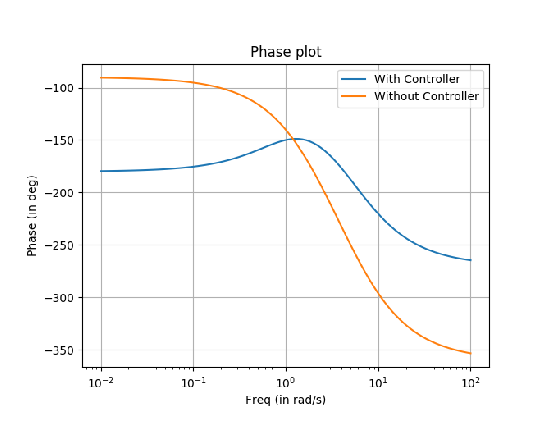
\includegraphics[width=\columnwidth]{./figs/ee18btech11021/EE18BTECH11021_PID.eps}
\caption{}
\label{fig:EE18BTECH11021_PID}
\end{figure}
\end{enumerate}
